\section{Results and Discussion}
We computed correctness of our DA subjects in identifying the missing information from DOI by using the Sorensen-Dice coefficient~\cite{sorensen1948method} and show these values in Figure~\ref{fig:Scatter}. We found that offline analysts were just slightly more accurate than real-time analysts, and generally both groups faired well. 

While not directly shown in Figure~\ref{fig:Scatter}, offline users were more accurate solving DA\_Task 4 (i.e., identifyng the recommended movie). The two groups differed in how they approached this task. Offline users searched their users' data to find the recommendation tasks, then picked one of the movies viewed towards the end of the task, since they were more likley to be an end-answer. Real-time analysts quickly identified when the recommendation task was underway and rushed to pick one of the first movies that their users considered. The real-time analysts also tended to be less accurate in detecting transitions between task. Finally, the offline users seemed more observant of the actual heatmap than real-time users, with real-time users reporting that they focused mainly on the vertically sorted labels on the sides of the heatmaps. 

While our preliminary results are promising we acknowledge that the number of concurrent users our analysts monitored was rather small. Even so, we provide a first account of how DOI eye-tracking can be used to enable real-time tracking of users' interests in data visualizations, thereby laying a foundation for applications described in section 1.  Moreover, we believe more complex visualizations, that borrow encoding principles and functionality from time-line and event monitoring applications, could allow analysts to track many users at once.  This is supported by one of our approach's main advantages: the ability to track users' eye-tracking data without having to look at the visual stimuli they viewed; this allows us to stack compact visualizations of multiple users' data, and pose complex computational queries. 


\begin{figure}[htb]
  \centering
  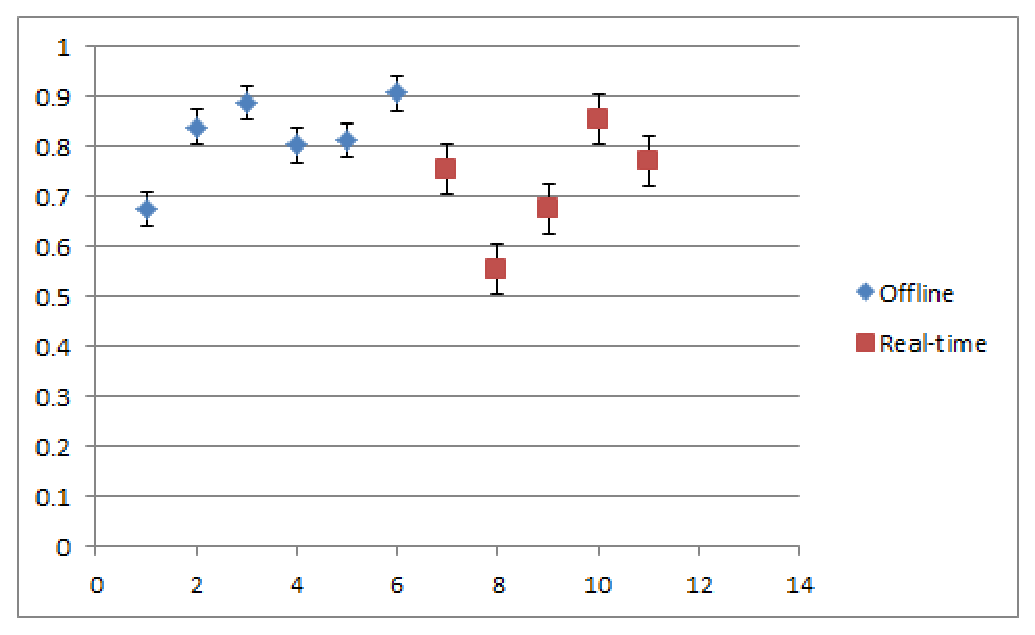
\includegraphics[width=0.9\linewidth]{images/Scatter.eps}
  \caption{Correctness of C-subjects in the C-study.}
	\label{fig:Scatter}
\end{figure} 

